
Lesen Sie das \emph{lshort}, zumindest inkl.\ Kapitel 2: \url{https://www.ctan.org/tex-archive/info/lshort/english/}!

Verwenden Sie explizite Zeilenumbrüche mit \lstinline[language=Tex]!\\! \emph{nur wenn unbedingt} nötig.

Für viele Anwendungsbeispiele wie das Einfügen von Abbildungen, Tabellen, Formeln und Formattierung allgemein schauen Sie sich das beiliegende Beispiel unter \texttt{./example} an.


Mögliche Kriterien:
The comparison investigates several aspects of each language, including program length, programming effort, runtime efficiency, memory consumption, and reliability
siehe:https://ieeexplore.ieee.org/abstract/document/876288

----------



--------------------

Wenn man über Applikationsentwicklung für mobile Endgeräte spricht, muss mann zwischen einigen verschiedenen Varianten unterscheiden.
1.Native Apps:
Native Apps sind Applikationen die mit der Plattformspezifischen Programmiersprache für die einzelnen Plattformen entwickeltwerden. Hierbei wird dann in Kotlin für Android oder Swift für iOS sowohl die UI als auch die Logik der App umgesetzt und ist so gesehen ein eigenständiges System, da die dadurch entwickleten Applikationen nur auf der Plattform genutzt werden können, für die sie geschrieben wurden.
Oft verfügen diese Applikationen auch noch über externe Schnitstellen, oder einer Verbindung zu einem Server, um etwa auf Datenhaltung oder andere Dienste zuzugreifen.
Ein Vorteil dieser Art der Entwicklung ist es, dass man sehr gut die verschiedenen Möglichkeiten der jeweiligen Plattform ausnutzen kann. So ist etwa eine Nutzung der Kamera in nativ entwickelten Applikation deutlich einfacher und besser umsetzbar. Dazu kommt, dass man bessere Nutzeroberflächen bauen kann, die auf die mobile Plattform angepasst sind.
Der Nachteil den eine Native Entwicklung jedoch hat ist der Aufwand und die damit verbundenen Kosten. Um für die beiden vorherschenden Plattformen eine Applikation anbieten zu können, braucht man die doppelte Zeit, als wenn man nur eine App entwickelt. Kommt dann noch eine Website und Serveranwendung oder ähnliches hinzu, wird schnell aus einer kleinen Anwendung ein großer Kostenproduzent.

2. Cross-Plattform-Apps
Unterscheidung zwischen Webview in App und z.B. Flutter 


3. Hybride Apps:
Hybride Apps sind Applikationen die zu gewissen Anteilen aus nativem Code bestehen und zu gewissen Teilen Code, Schnitstellen oder Darstellungen anderer Websiten bzw. Webapplikationen nutzen. Der häufigste Anatz ist es hier, Webappplikationen zu einem gewissen Anteil in einem Frame der Applikation darzustellen und dabei einzelne Seiten durch nativ entwickelte Oberflächen zu ersetzen und die Daten an die Webapplikationen weiter zu geben. 



-----
Vortrag zu Cross Plattform Notizen:

\begin{figure}[ht]
  \centering
  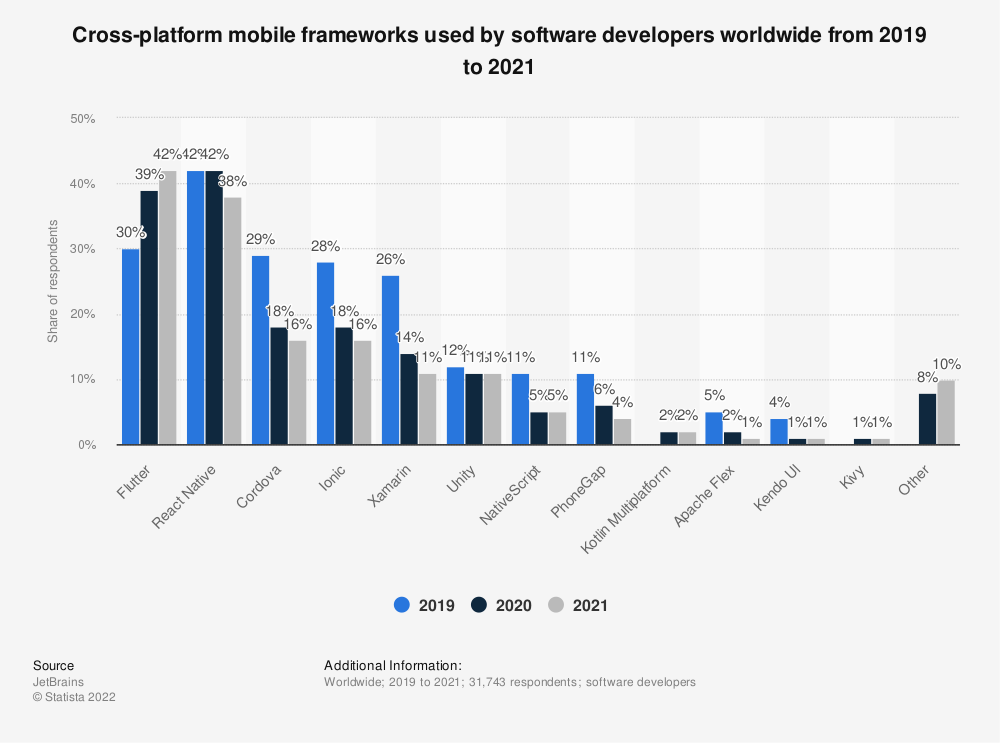
\includegraphics[height=7cm,keepaspectratio]{images/cross-platform-mobile-frameworks.png} 
  \caption{Cross-Plattform-Frameworks 2019-2021}
  \label{fig:statista_cross_plattform}
\end{figure}

Abbildung \ref{fig:statista_cross_plattform} zeigt Statistik von JetBrains die Verteilung von verschiedenen Sprachen zeigt:
 -> Flutter vielversprechend
 
Flutter ist für Ubuntu Standardsprache zur Desktopanwendungsentwicklung

Mittlerweile für fast alle möglichen Plattformen übersetzbar und Gemeinschaft sehr aktiv.

Es gibt eigentlich keine richtigen Gründe mehr nativ zu entwickeln. Mit Flutter ist quasi alles umsetzbar, was man will und wenn es noch nicht das benötigte Plugin gibt, so kann man es selbst entwickeln. Das kann zwar etwas kompliziert werden, aber von der Sache her nicht ummöglich.

Bei Flutter kann man Plugins schreiben. Diese funktionieren, indem man einen Dart Code schreibt und die entsprechenden nativen Codeteile. Dadurch weiß der Dart-Compiler wie er den DartCode in die verschiedenen nativen Anwendungen übersetzt.

Die Grundfunktionalität von Flutter funktioniert, indem ein Canvas genommen wird, auf den die verschiedenen UI-Komponenten "drauf" gemalt werden. Mit einer dahinter liegenden Zuordnung und Tracking wird es dann zu einer funktionalen Nutzeroberfläche.

--------

Frage: Ist es überhaupt noch sinnvoll, eine App nativ zu entwickeln? Macht es nicht immer mehr Sinn eine Cross-Plattform-Entwicklung zu tun, falls man einmal doch auf eine weitere Plattform umsteigen will? 
Es könnte ja immer sein, dass man die App erweitern kann. Dann müsste man eine zusätzliche Entwicklung bezahlen. Man müsste gewissermaßen komplett von vorne anfangen. Während wenn man bereits in Flutter etwa entwickelt hat, muss man nur noch die benötigte Plattform kompilieren und eventuell ein paar Sachen anpassen. 

Andererseits hat man einen schnell sich ändernden Technologiemarkt. Flutter wurde erst 2017 auf den Markt gebracht und ist 2021 zum Führenden Framework aufgestiegen. Andererseits ist React Native von einem der viel versprechendsten Frameworks seit dem Erscheinen von Flutter auf dem Abeseigenden Mast und andere haben ganz und gar Ihre Bedeutung verloren.Etwa Apache Flex. Das auch seit 2017 nicht mehr weiter entwickelt wird. So zeigt sich, dass die Wahl auf das richtige Framework und die richtige Entwicklungsstrategie eine sehr wichtige ist und mit viel Vorsicht getroffen werden muss.

-----
Flutter:
Flutter ist ein von Google entwickelte Programmiersprache die mittlerweile das bedeutendste Framework in der Cross-Plattform Entwicklung. Das spannende an dieser Plattform ist, dass nicht nur Google, eines der wichtigsten Technologieunternehmen dahintersteht, sondern ist ebenfalls sehr stark in der Entwicklung mit ständiger Weiterentwicklung. Es entstehen außerdem immer neue Tools und es werden mehr und mehr Plugins angeboten, um die Entwicklung einer Flutter App noch einfacher zu machen und dabei jede mögliche Funktionalität verfügbar anzubieten.

------
Vielleicht ist es gar nicht so sonnvoll feste Kriterien zu finden an denen man die Entwicklung an sich bewerten kann, sondern eher das Endergebnis. Es ist ja auch keine Bewertung sondern eher ein Vergleich.
Kriterien sind:
-Programmlänge
-Programmieraufwand
-Laufzeit effizienz
-Speicherplatzverbrauch
- verfügbarkeit

-Verfügbarkeit von Hilfestellungen und Fragen und Antworten

- Code lesbarkeit[1]
- Einfachheit[1]
- Datentypen[1]
- Syntax[1]
- Designed to make it impossible to making (some) stupid mistakes? [1]
- Programmierfähigkeiten während Entwicklung ohne ständiges neu Compilen und schnelles Testen     von Sachen[1]
- Possibilitys for reusability and dry code[1]
- A language may be wonderful and amazing and increase developer productivity, but if no talented people are out there that know the language, how will you hire the best team?[1]

- Support for internationalization [2]

- Keine Änderung von Grundsätzlichen Strukturen und Funktionalitäten.

- In general, we think you can write good software in Java, C\#, Python, PHP, or any other myriad languages. You can also write really bad software using any of those. To us, the adherence to widely accepted design principles and philosophies is more important than the specific language.[3]



Quellen hierzu:
-Medium Leseliste
-[1] https://cs.lmu.edu/~ray/notes/evaluatingprogramminglanguages/  , Loyola Marymount University website
-[2]https://easyexamnotes.com/p/language-evaluation-criteria-ppl.html
-[3] https://www.27global.com/how-to-choose-a-programming-language/
- [4]https://journals.plos.org/plosone/article?id=10.1371/journal.pone.0088941
- [5]\url{https://books.google.de/books?id=XUqqCAAAQBAJ&lpg=PR6&dq=criteria%20for%20evaluating%20programming%20languages&lr&hl=de&pg=PA35#v=onepage&q&f=false}

------
Framework Kriterien:

Quellen:
- [1] https://symfony.com/ten-criteria
- [2]


- Popularität und Community Größe: Je mehr genutzt und bekannt, umso mehr evolution und besserwertige und mehr Plugins und Lösungen [1]

- Philosophy: Ein von Profis für diesen Zweck entwickeltes Framework passt besser zu eigenem Projekt während Entwicklung für Framework für sehr spezielle Sachen eher unnützlich [1]

- Langlebigkeit: Wenn ein Framework kurz vor Ende ist oder schon lange keine Updates mehr erhalten hat, so wird es eventuell keine Große Hilfe im meistern zukünmftiger Probleme sein [1]

- Technische Details: Frameworks, die sich an die technischen Standards halten, helfen, nicht zu sehr an speziellen Lösungen eines Frameworks hängen zu bleiben und auch offen für neue Programmiersprachen und Frameworks zu bleiben [1]

- Sicherheit: Frameworks müssen bestimmte Sicherheitsrichtlienien erfüllen. [1]

- Gute Dokumentation: Eine gute Dokumentation durch den Entwickler ist entscheidend um verlässliche Informationen zu erhalten [1]

-Lizenzen: Bei Programmiersprachen wie Java gibt es einige Versionen die nur mit gekaufter Lizenz nutzbar sind. Darüber sollte man sich klar machen, bevor man eine Entscheidung trifft. Es ist grundsätzlich kein schlechtes Zeichen, muss allerdings beachtet werden. [1]

- Entwicklerverfügbarkeit [1]

-Ausprobieren: Wenn man nicht mit dem Framework zurecht kommt, sollte man eventuell ein anderes versuchen. Nur durch ausprobieren erfährt man wie gut man damit entwickeln kann. [1]
